\documentclass[tikz,border=2pt]{standalone}
\usepackage{amsmath}
\usepackage{pgfplots}
\pgfplotsset{compat=1.18}
\usetikzlibrary{arrows.meta}
\begin{document}
% An atomic vector is a row of cells with positions 1, 2, ...; c(x, y) copies the values of x
% and then of y into one new vector of length 6.
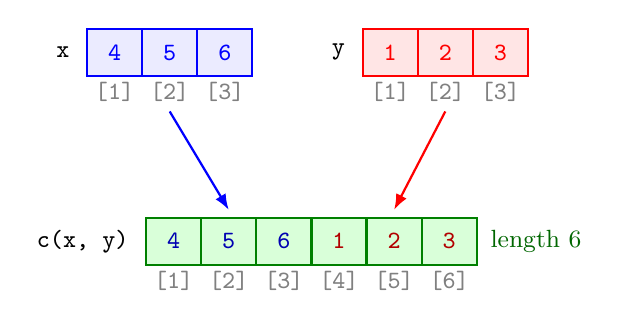
\begin{tikzpicture}[font=\small, >={Latex[length=2mm]},
  cell/.style={draw, thick, minimum width=7mm, minimum height=6mm, inner sep=0pt, font=\small\ttfamily}]
  % x
  \node[anchor=east] at (-0.1,2.4) {\texttt{x}};
  \foreach \v [count=\i] in {4,5,6} {
    \node[cell, blue, fill=blue!8] at (0.7*\i-0.35,2.4) {\v};
    \node[gray, font=\small\ttfamily] at (0.7*\i-0.35,1.9) {[\i]};
  }
  % y
  \node[anchor=east] at (3.4,2.4) {\texttt{y}};
  \foreach \v [count=\i] in {1,2,3} {
    \node[cell, red, fill=red!10] at (3.5+0.7*\i-0.35,2.4) {\v};
    \node[gray, font=\small\ttfamily] at (3.5+0.7*\i-0.35,1.9) {[\i]};
  }
  % combined
  \node[anchor=east] at (0.65,0) {\texttt{c(x, y)}};
  \foreach \v/\c [count=\i] in {4/blue,5/blue,6/blue,1/red,2/red,3/red} {
    \node[cell, draw=green!50!black, fill=green!15] at (0.75+0.7*\i-0.35,0) {\textcolor{\c!70!black}{\v}};
    \node[gray, font=\small\ttfamily] at (0.75+0.7*\i-0.35,-0.5) {[\i]};
  }
  \draw[->, thick, blue] (1.05,1.65) -- (1.8,0.4);
  \draw[->, thick, red] (4.55,1.65) -- (3.9,0.4);
  \node[green!40!black, anchor=west] at (5.0,0) {length 6};
\end{tikzpicture}
\end{document}
